\chapter{Recommendations}\label{sec:recommendations}
In this chapter, we will give some pointers for both the back-end and the front-end as to how the system can be extended and improved.
%For future improvements on this project one might decide upon two ways to do this. The first is to look at the requirements which have not yet been fulfilled and fulfil those. Depending on the needs of the user one might want to implement different things. For extending the application to international places one would want to use data from top-level domains other than .nl. However others might be interested in finding different relations, for which one would need to have other training data.
%If one has more time it might be interesting to instead of using a classification algorithm, to choose a clustering algorithm. \todo{extend}

\todo{ Make recommendations for future version, for extending the back-end and front-end
 Try to mention the requirements here}
 
\section{Extending the Back-End}
In this section, we present several recommendations to improve the back-end.

\subsection{Extending the Data Set}
The input data is now limited to dutch documents only. This limits the amount of available data and also limits the network of cities that can be extracted from this data. In a future version it will be interesting to be able to parse other languages as well, starting with English. This would require some investigation regarding stop-words in English and what primarily causes false positives for semantic association of cities in English documents. Next to that, in a future version of the application it would be interesting to be able to use other data than Common Crawl data. This would require a few modifications to the data storage functions because a unique identifier per stored document is needed. These modifications should lead to an application that is able to use a lot more data to find relations between cities, which in turn should lead to more reliable and credible results.


\subsection{Improving Document Filtering}
Other than the required co-occurrence of cities, there is little noise cancelling in documents. Some documents contain lists of cities and are cancelled out as explained in section \ref{sec:filtering_docs}. However, there might be more intuitive ways for better document filtering. One could for example discard the contents of specific HTML elements, such as forms and input fields. Moreover, some kind of domain blacklist could be constructed to filter out entire (sub)domains that are known to contain mostly false-positives. For example, the client mentioned that many pages of Airbnb were reviews from people of all over the country, but represent no relation between these locations. Another way to extend the document filtering is to have some way to allow for city aliases. By doing so, more documents will pass the filtering stage so more relations can be extracted.

\subsection{Constructing More Advanced Classifiers}
While our classifier achieves a reasonable mean accuracy of 75\%\-80\% \ref{sec:mean-accuracy}, these results can be improved further to reach a even higher mean accuracy. Below we will explain what we see as potential improvements to the classifier.

\subsubsection{Data Set}
Our first recommendation is to keep expanding the data set. This will lead to a more accurate classifier. The classification interface can be used for this task. This way the data set can keep getting expanded over time.
\subsubsection{Parameter Optimisation}
The estimator algorithm that we use in our Scikit \texttt{Pipeline} takes a number of parameters that effect the outcomes we get back from the classifier. These parameters can be tuned as described in \footnote{\url{http://scikit-learn.org/stable/modules/grid_search.html}}. These parameters, so called hyper-parameters, .....
\subsubsection{Empirical Tests of Classifiers}
Besides these two options it would be a good idea to implement more algorithm specific \texttt{ModelManagers} and to compare the results of these different classifiers on our data set. This way we could make sure we always select the most accurate classifier when running the classification over our downloaded documents.\\
Another improvement concerning the classifier would be to try out binary classifiers instead of a multi-value classifier which we currently use. A binary classifier is a classifier that takes positive inputs and negative inputs and can decide if an unseen input is in that specific class or not. This means we would generate a binary classifier for every category that we have and run a document through every binary classifier after which we would select the category or categories to which this document belongs. An multi-value classifier on the contrary can label an input with multiple classes, or categories in our case\cite{hess2008multi}.  

\subsection{Upgrading the Server}
\todo{@Piet}
As discussed in section \ref{sec:Discussion - Open Issues}, multiple open issues are due to the server we used, which is not as powerful as we would have liked. For future versions, the server should be upgraded to at least 16GB RAM and preferably at least 8 CPUs, to allow for more efficient multiprocessing and to be able to keep the database in memory for much faster reading. Additionally, an SSD instead of HDD would greatly improve the database speed for both reading and writing. To speed up database access even more, it would help to have a dedicated physical server that only runs the database.

\subsection{Building a Command Line Interface}
The delivered application provides an API and a visual interface, however, there is no command-line interface yet. If a user knows how to program Python it would be possible to call functions using the Python interpreter, but this is far from ideal. A future version could have a CLI (Command-Line Interface) that makes calling parts of the system fairly straightforward. For example, this would enable a user to call just the filtering subsystem or just the classification functionality on one or more documents. Next to that, the user could also change and run a separate configuration locally to experiment with parts of the application without changing the configuration of the application running on a server.

\section{Extending the Front-End}
An improvement in the front end that could add great value to the system, would be an interface that lets users manipulate classifiers and data sets. The interface should allow user first of all to select which classifier is used as the default classifier for the system. Besides that allowing a user to adjust parameters of the classifier in the interface and subsequently running accuracy tests that get displayed clearly, would add a lot of flexibility and value to the system.\\
Furthermore viewing and editing the data set associated to an classifier and/or category would allow for validation by human users of the system and for quick adjustments if for example a document would be added to a wrong category by accident.\\
Finally we would recommend to look for better solutions of displaying relations on the map. Now if we show many cities and relations the map basically becomes a incomprehensible clutter of lines, as show in figure \ref{fig:incomp-map}.

\begin{figure}[H]
\centering
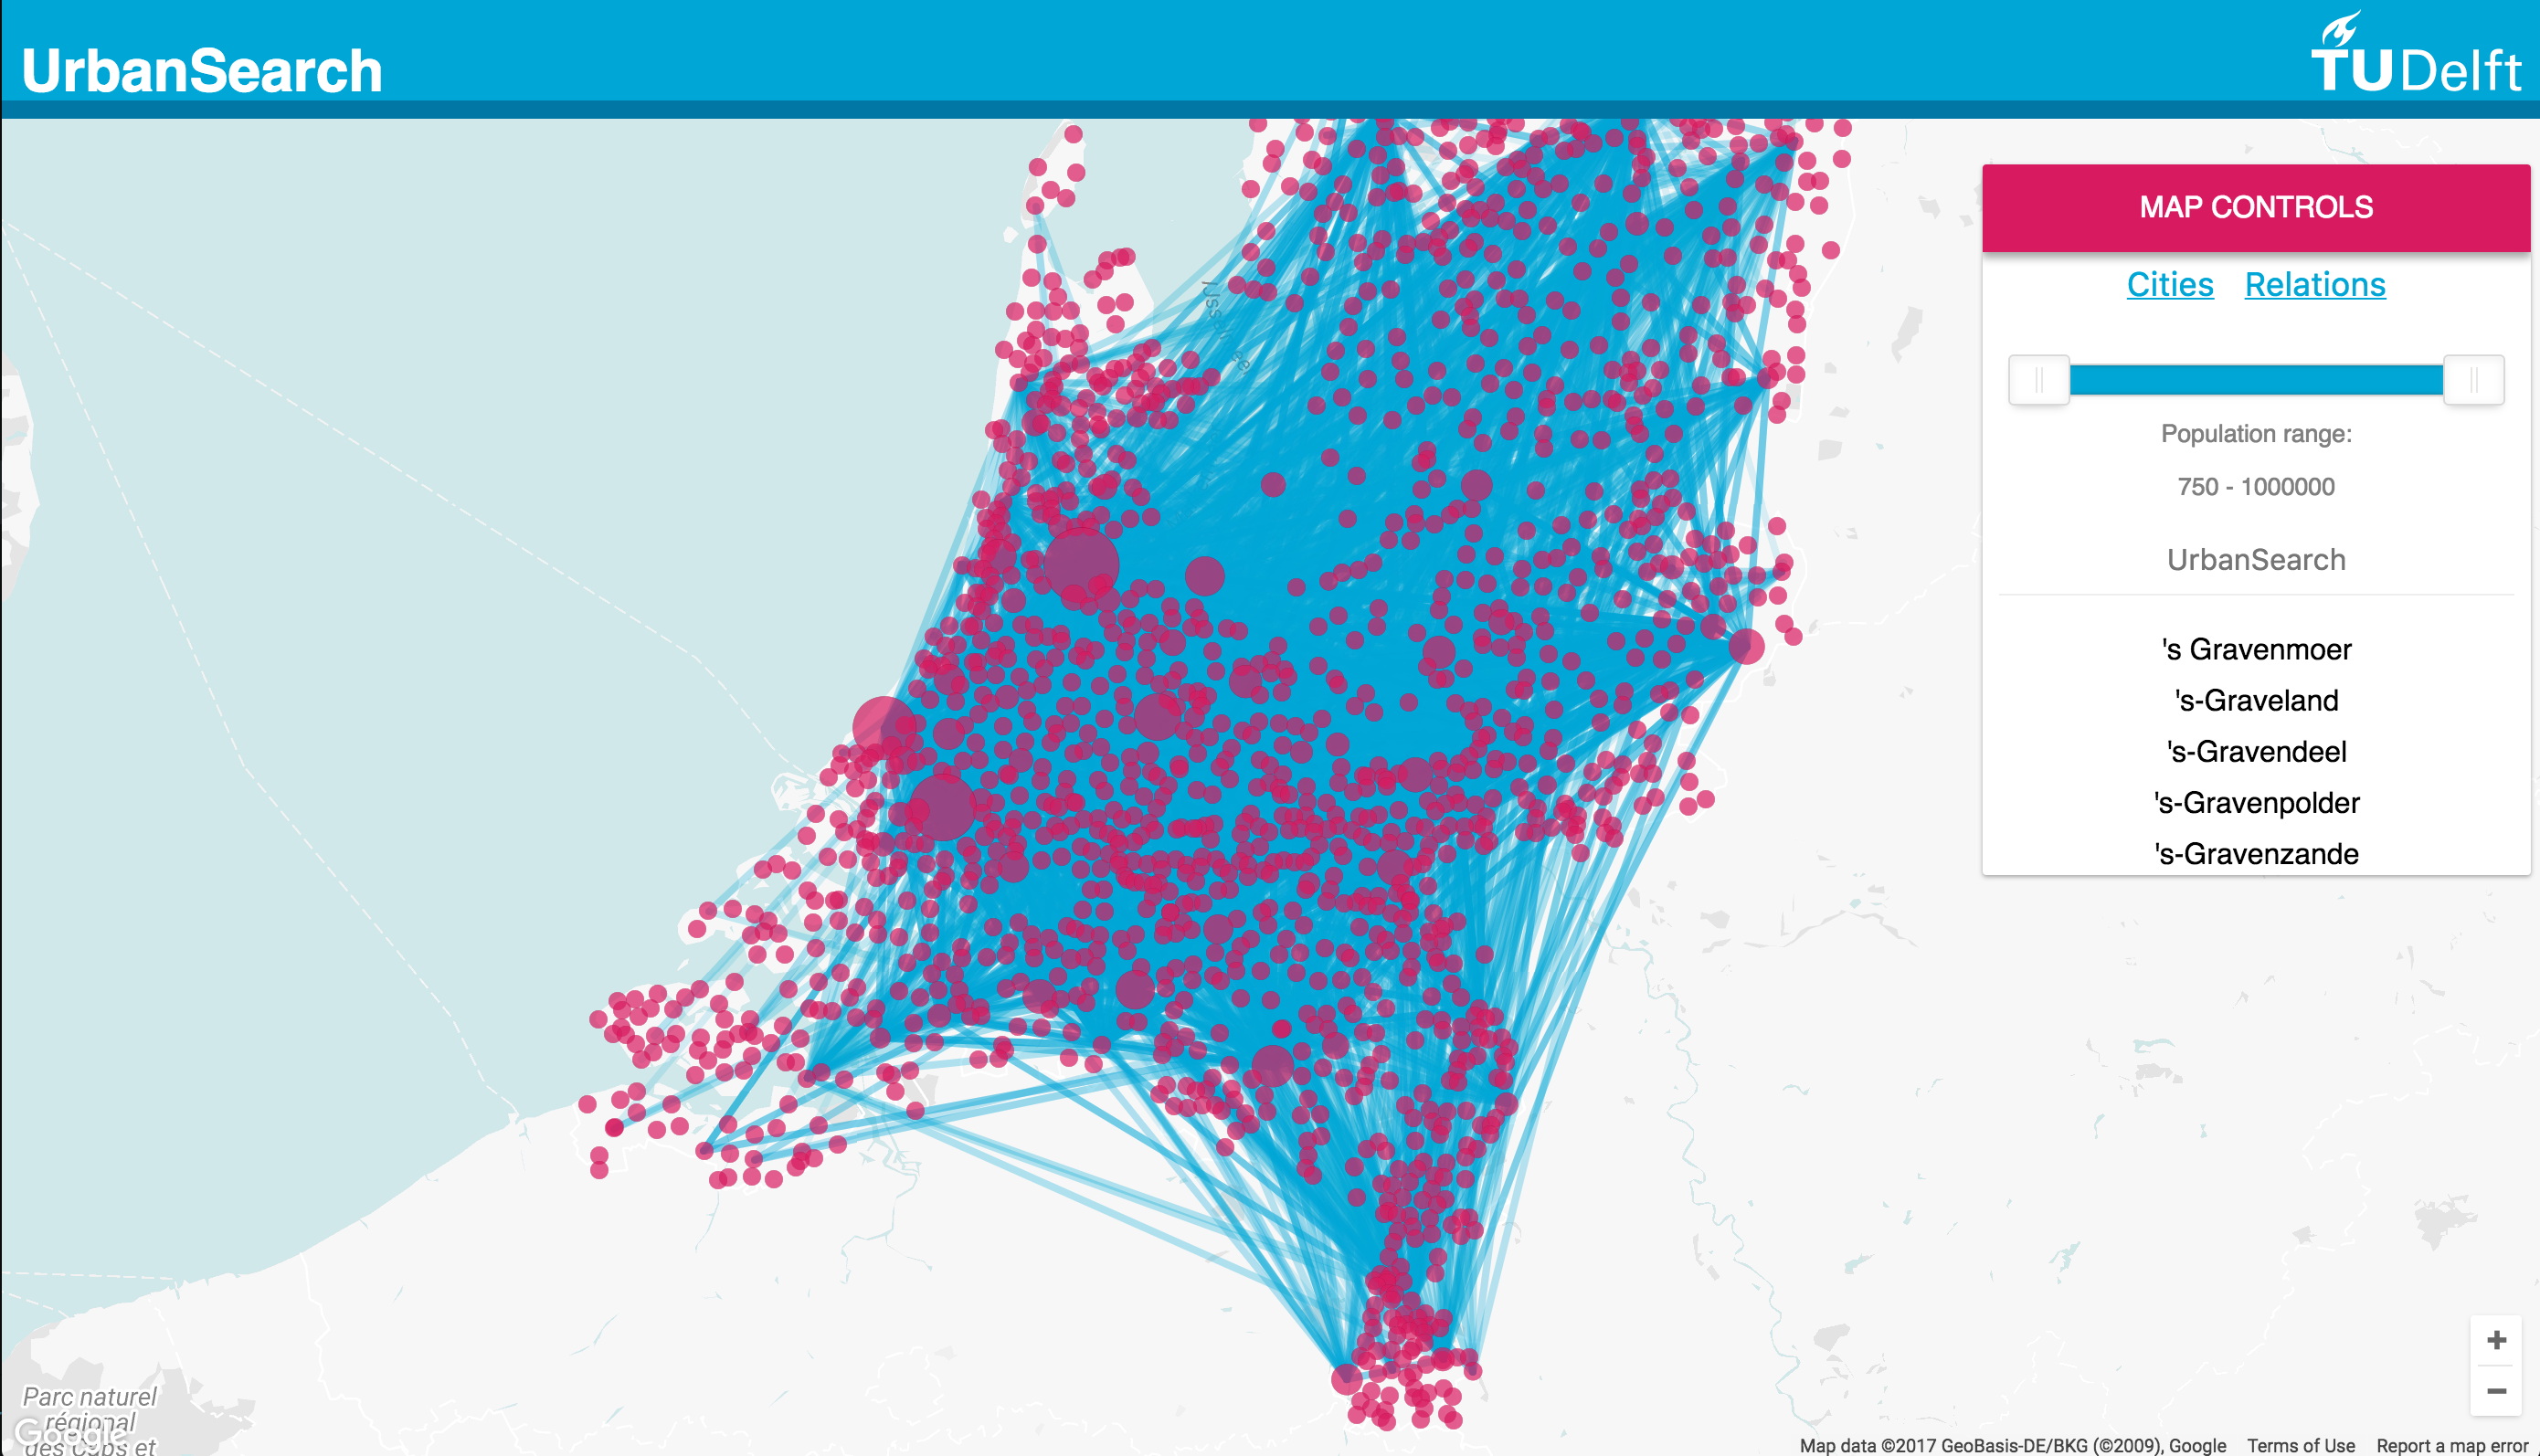
\includegraphics[width=0.8\textwidth]{incomp-map}
\caption{Example of map clutter}
\label{fig:incomp-map}
\end{figure}